\subsubsection{Hessian profiling analysis}
\label{sec:hessianprofiling}

In order to complement the results obtained
with the Bayesian reweighting approach,
we can also use a profiling method, suitable
for Hessian PDF sets, to estimate the effect of including
lattice-QCD pseudo-data into the fit. 
%
Specifically, we
choose the HERAPDF2.0 as a representative set of Hessian PDFs, and 
we have used the same Lattice data on moments to estimate the impact
on the HERAPDF2.0 unpolarized Hessian PDFs~\cite{Abramowicz:2015mha}. 
%
An additional advantage of the HERAPDF2.0 is that they use
$\Delta\chi^2=1$ for defining the Hessian error PDFs which ensures a
one to one correspondence of the profiling and reweighting methods.

In case of Hessian PDF sets, the Hessian profiling method
can be used to both check the compatibility of new data on a given PDF set,
and also  estimate the impact these data will have on the PDFs. 
In the following we describe essential components of the profiling method, 
and will assume  that the considered Hessian PDF set is using tolerance of $\Delta\chi^2=1$ 
which corresponds to 68\%~CL uncertainties.

The central values of the considered moments are obtained using the central PDFs and the corresponding
errors are calculated according to:
\begin{equation}
\delta\mathcal{F}_i = \frac{1}{2} \sqrt{\sum_{k}\left(\mathcal{F}_i(f_k^+)-\mathcal{F}_i(f_k^-)\right)^2},
\quad i=1,\ldots,N_{\rm mom}
\end{equation}
where $k$ numbers the error PDFs.
%
In the profiling method we consider a $\chi^2$ function in which the $\chi^2$ of the new
data has been added to the initial $\chi^2$:
\begin{equation}
\label{eq:newchi2}
\chi^2_{\text{new}} = \chi_0^2 + \sum_{k}^{N_{\text{eig}}} z_k^2
                    + \sum_{i=1}^{N_{\text{data}}}
                      \frac{\lp \mathcal{F}_i - \mathcal{F}_i^{\rm(exp)}\rp^2}
                           {\lp\delta\mathcal{F}_i^{\rm(exp)}\rp^2}
\end{equation}
where $\chi^2_0$ is the value of the $\chi^2$ function in the minimum of the initial PDF set,
$z_k$ are parameters diagonalizing the Hessian matrix of the initial PDF set,
$N_{\text{eig}}$ is the dimension of the eigenvector space in which initial Hessian errors are defined
(half of the number of error PDFs), $\mathcal{F}_i^{\rm(exp)}$ is the new data,
and $\mathcal{F}_i$ the corresponding theory prediction.

In the spirit of the Hessian method the new theory predictions $\mathcal{F}_i$ can be expanded
using a linear approximation:
\begin{equation}
\mathcal{F}_i \simeq \mathcal{F}_i[S_0] + \sum_k \frac{\partial\mathcal{F}_i[S]}{\partial z_k}\bigg|_{S=S_0} z_k \quad
              \simeq \mathcal{F}_i[S_0] + \sum_k D_{ik} w_k \ ,
\end{equation}
where $S_0$ represents central PDF and $D_{ik}=\frac{1}{2}(\mathcal{F}_i[S_k^+]-\mathcal{F}_i[S_k^-])$;
here the  derivative has been approximated by a finite difference of the 
Hessian PDF error sets $S_k^{\pm}$.
%
The new $\chi^2$ of Eq.~\eqref{eq:newchi2} can now be minimized with respect to the parameters $w_k$,
which results in:
\begin{equation}
\boldsymbol{\vec{w}_{\text{{\bf min}}}} = \boldsymbol{-B^{-1}} \boldsymbol{\vec{a}},
\end{equation}
with
\begin{equation}
%\begin{split}
B_{kn} = \sum_i \frac{D_{ik}D_{in}}{\lp\delta\mathcal{F}_i^{\rm(exp)}\rp^2} + \delta_{kn},
%\\
\qquad
\qquad
a_k = \sum_i \frac{D_{ik}(\mathcal{F}_i[S_0] - \mathcal{F}_i^{\rm(exp)})}{\lp\delta\mathcal{F}_i^{\rm(exp)}\rp^2} \ . 
%\end{split}
\end{equation}
%
The components of the solution $\boldsymbol{\vec{w}_{\text{{\bf min}}}}$ define a new set
of PDFs representing a global minimum after including the new data:
\begin{equation}
f_{\text{new}} = f_{S_0} + \sum_{k=1}^{N_{\text{eig}}} \frac{f_{S_k^+}-f_{S_k^-}}{2} w_k^{\text{min}} \ .
\end{equation}
At the same time $\boldsymbol{\vec{w}_{\text{{\bf min}}}}$ also  defines  a penalty term 
\begin{equation}
P = \sum_{k=1}^{N_{\text{eig}}} \lp w_k^{\text{min}} \rp^2
\end{equation}
which can be used to estimate whether the new data is consistent with the initial set of PDFs;
a penalty of $P\ll1$ means that the new data is consistent.
%
Finally, a set of new error PDFs can be also defined; in this case matrix $B_{kn}$ plays the role of
the Hessian matrix from which the PDF errors can be obtained. 

We have performed this study assuming the same 3 scenarios for the errors of the Lattice data,
{\it cf.,}~Table~\ref{tab:scenarios}. 
The study was performed using the xFitter program~\cite{Alekhin:2014irh}.
%
The results of the profiling are shown in Table~\ref{tab:unpolmomentsProf} where the uncertainties
of the considered moments are displayed for the case of the initial HERAPDF2.0 PDF and after including the Lattice
moments data in the three scenarios.
%
%
Additionally, in Fig.~\ref{fig:pdfsProf}, we show the impact of the Lattice data on the PDFs by
comparing the relative errors of the PDFs in scenarios A, B and C with initial HERAPDF2.0 errors.

%%%%%%%%%%%%%%%%%%%%%%%%%%%%%%%%%%%%%%%%%%%%%%%%%%%%%%%%
\begin{table}[h]
  \centering
  \renewcommand{\arraystretch}{1.3} 
\begin{tabular}{c||c|c|c|c}
  \hline &  Original  & Scen A  &  Scen B  &  Scen C  \\
  \hline
  \hline
  $\la x\ra_{u^+}$     &  $0.3720\pm 0.0036$  &  $0.3720\pm 0.0030$  &  $0.3720\pm 0.0027$  &  $0.3720\pm 0.0020$ \\
  $\la x\ra_{d^+}$     &  $0.1845\pm 0.0053$  &  $0.1845\pm 0.0028$  &  $0.1845\pm 0.0023$  &  $0.1845\pm 0.0015$ \\
  $\la x\ra_{s^+}$     &  $0.0346\pm 0.0037$  &  $0.0346\pm 0.0015$  &  $0.0346\pm 0.0012$  &  $0.0346\pm 0.0009$ \\
  $\la x\ra_{g}$       &  $0.4006\pm 0.0078$  &  $0.4006\pm 0.0042$  &  $0.4006\pm 0.0035$  &  $0.4006\pm 0.0024$ \\
  $\la x\ra_{u^+-d^+}$ &  $0.1875\pm 0.0074$  &  $0.1875\pm 0.0045$  &  $0.1875\pm 0.0039$  &  $0.1875\pm 0.0027$ \\
  \hline
\end{tabular}
\caption{\small Values of the unpolarized PDF moments
  used as pseudo-data, as well as the corresponding results
  after the profiling  for the
three scenarios summarized in Table~\ref{tab:scenarios}.
%
The HERAPDF2.0 PDFs were used, and the PDF uncertainties quoted correspond in all cases to 68\%~CL intervals.
\label{tab:unpolmomentsProf}
}
\end{table}
%%%%%%%%%%%%%%%%%%%%%%%%%%%%%%%%%%%%%%%%%%%%%%%%%%%%%%%%



%%%%%%%%%%%%%%%%%%%%%%%%%%%%%%%%%%%%%%%%%%%%%%%%%%%%%%%%
\begin{figure}[!t]
\centering
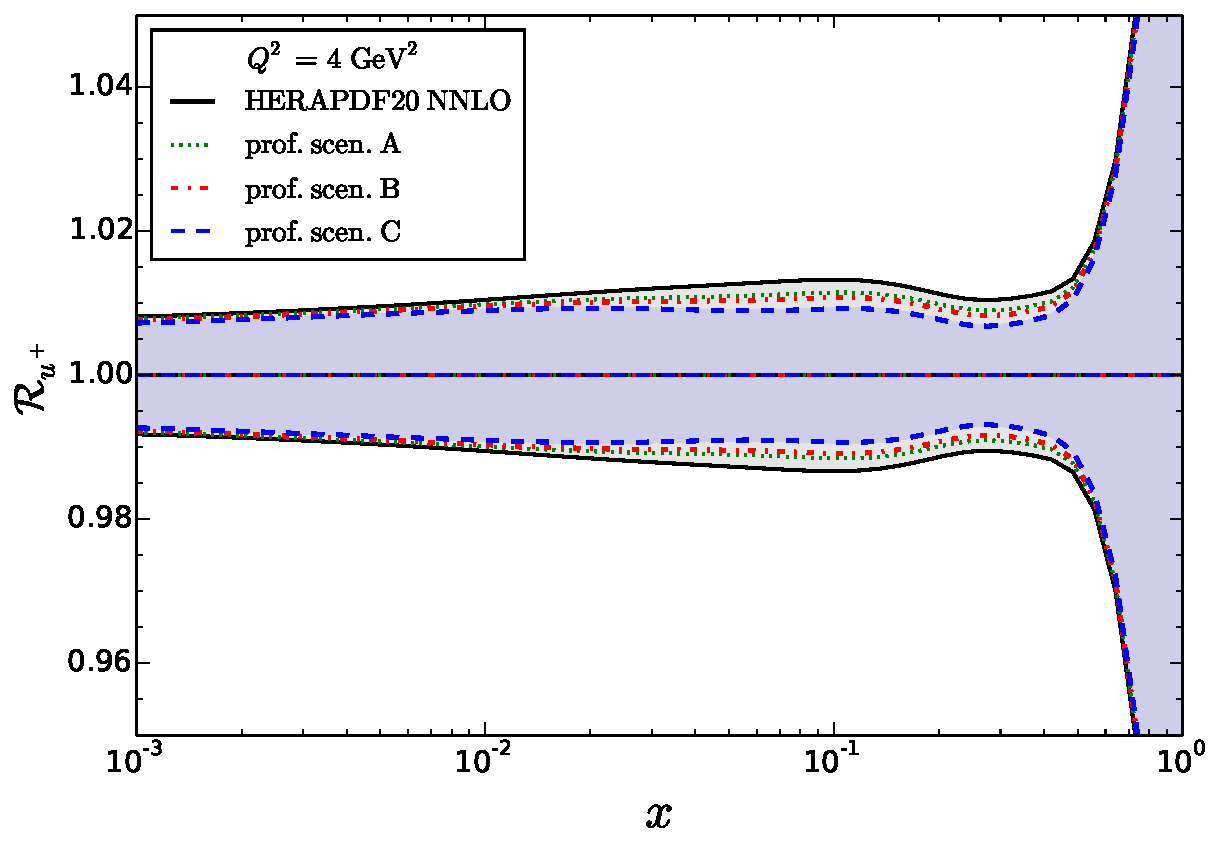
\includegraphics[width=0.45\textwidth]{plots/ratio_uPubar_Q2.pdf}
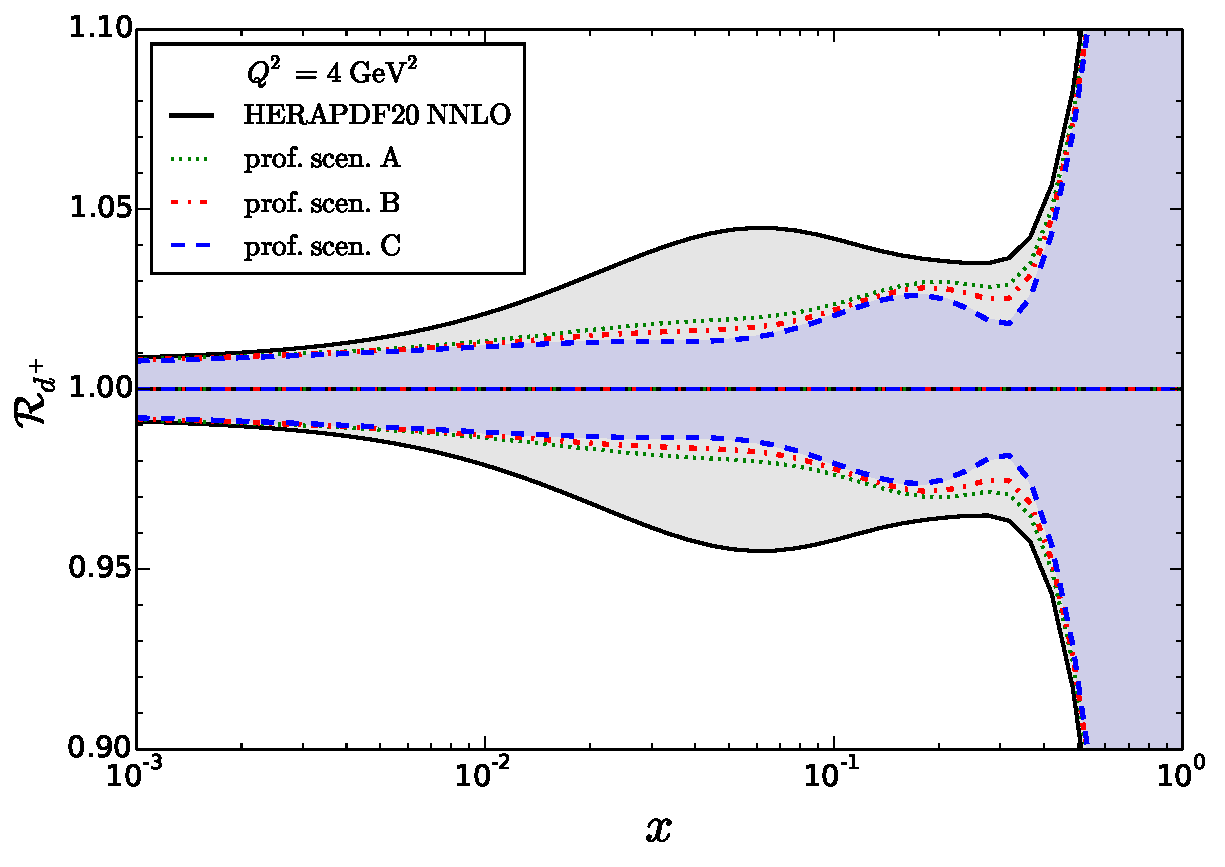
\includegraphics[width=0.45\textwidth]{plots/ratio_dPdbar_Q2.pdf}\\
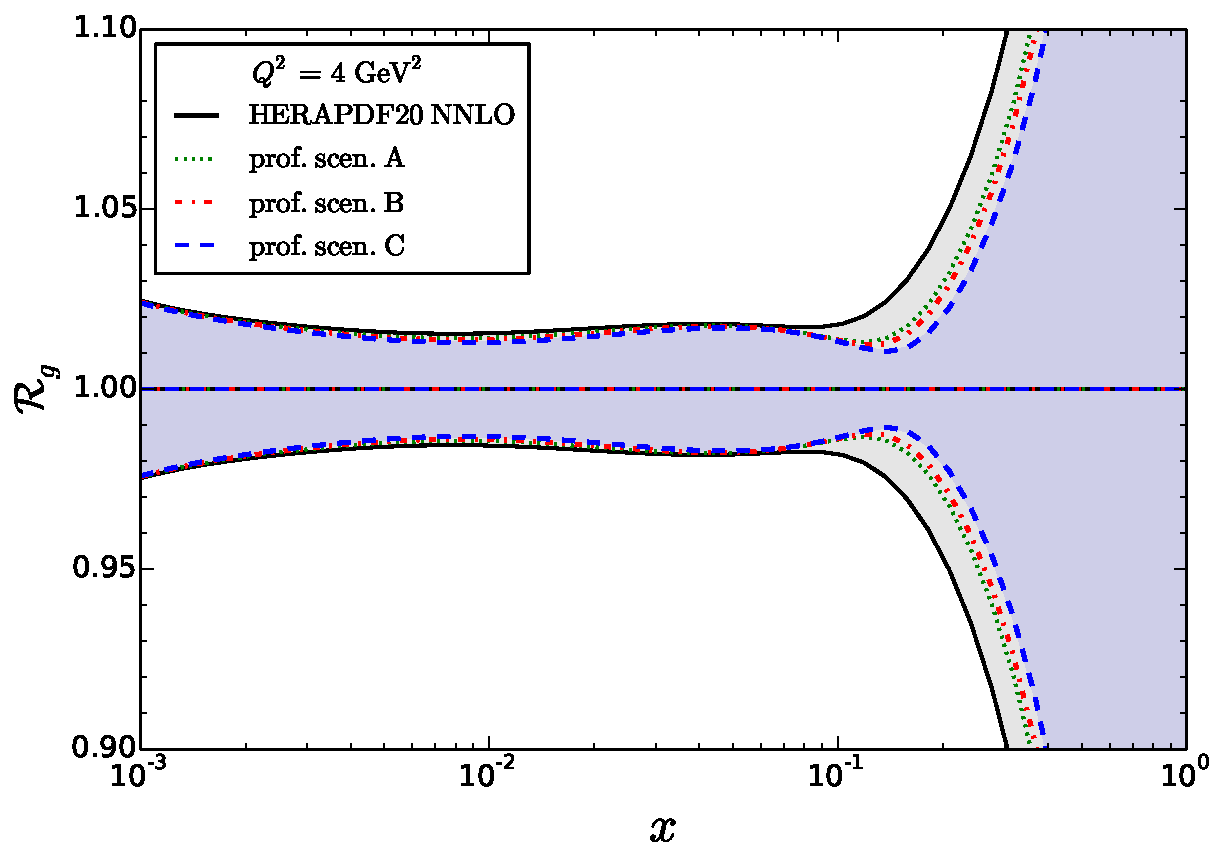
\includegraphics[width=0.45\textwidth]{plots/ratio_g_Q2.pdf}
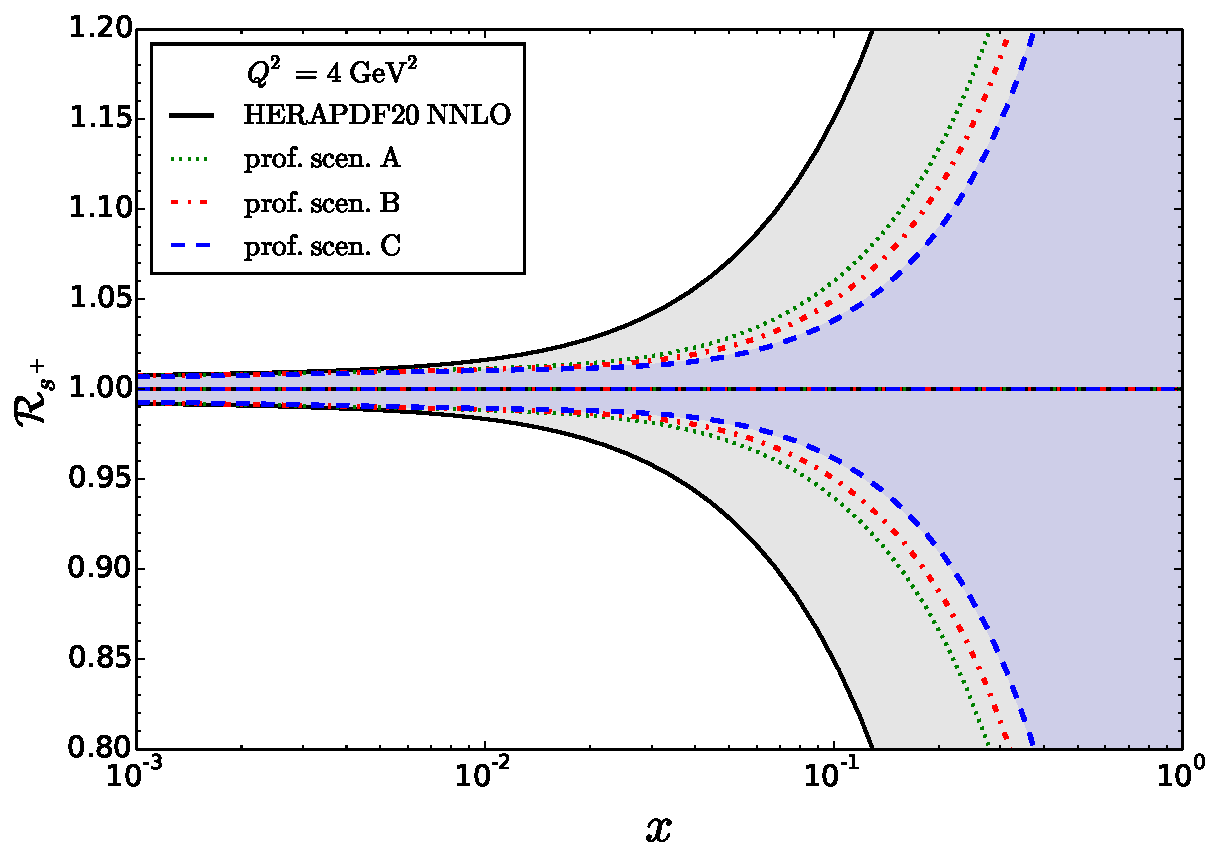
\includegraphics[width=0.45\textwidth]{plots/ratio_sPsbar_Q2.pdf}
\caption{\small Combinations of PDFs: $u^+$, $d^+$, $g$, $s^+$ at scale $Q^2=4$ GeV$^2$
for initial HERAPDF2.0 compared with the PDFs resulting from including Lattice moments
data in scenarios A, B and C.}
\label{fig:pdfsProf}
\end{figure}
%%%%%%%%%%%%%%%%%%%%%%%%%%%%%%%%%%%%%%%%%%%%%%%%%%%%%%%%

